\begin{frame}{Vergleich aller Modelle: Red20-Vorauswahl}
\tiny
\begin{tabularx}{\textwidth}{l r r r r X}
\toprule
Modell & GT-Faces & Treffer & Recall & ms/Bild & Rolle nach Vorauswahl \\
\midrule
FCOS red20 ep1 & 3.443 & 1.884 & 0,547 & 36,2 & Recall-Gewinner \\
Faster R-CNN red20 ep1 & 3.443 & 1.714 & 0,498 & 51,4 & starker dritter Kandidat \\
YOLOv8m red20 ep1 & 3.443 & 1.399 & 0,406 & 43,7 & Pipeline-Gewinner \\
RetinaNet red20 ep1 & 3.443 & 1.125 & 0,327 & 35,0 & faellt wegen Recall ab \\
\bottomrule
\end{tabularx}
\vspace{0.35em}
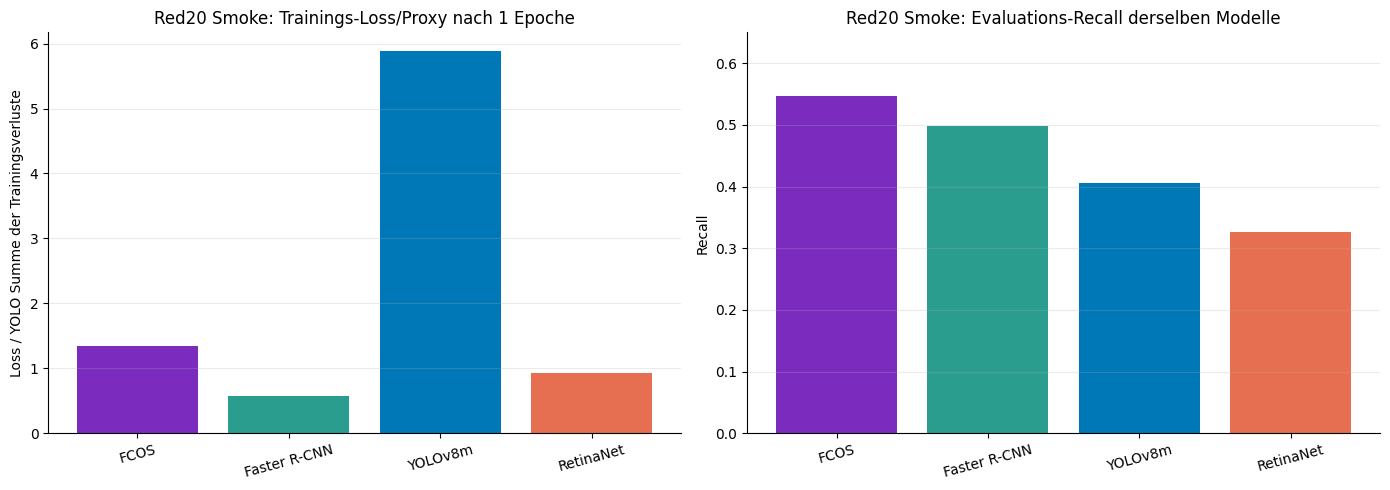
\includegraphics[width=\textwidth,height=0.35\textheight,keepaspectratio]{imglib/face_model_lab/red20_training_vs_eval.png}
\vspace{0.25em}
\scriptsize
\begin{itemize}
    \item Erster Block: alle Modelle auf gleicher reduzierter Trainingsbasis.
    \item Gewinner fuer den vertieften Lauf: FCOS als Recall-Sieger, YOLOv8m als Pipeline-Sieger.
    \item Faster R-CNN wird zusaetzlich in den finalen Vergleich aufgenommen, weil der Red20-Recall stark genug ist.
\end{itemize}
\end{frame}

\begin{frame}{Finaler Vergleich: Gewinner plus neuer RCNN-Lauf}
\tiny
\begin{tabularx}{\textwidth}{l r r r r X}
\toprule
Modell & GT-Faces & Treffer & Recall & ms/Bild & Interpretation \\
\midrule
FCOS ResNet50-FPN red6 ep10 & 5.015 & 3.375 & 0,673 & 34,9 & bester Recall \\
YOLOv8m red6 ep10 & 5.015 & 2.283 & 0,455 & 14,6 & schnellster Pipeline-Kandidat \\
Faster R-CNN MobileNetV3-FPN red20 ep1 & 5.015 & 1.829 & 0,365 & 620,6 & kuehler, aber schwach und langsam \\
\bottomrule
\end{tabularx}
\vspace{0.4em}
\begin{itemize}
    \item Evaluation: 500 Validierungsbilder, 5.015 Ground-Truth-Gesichter, IoU 0,4, Confidence 0,25.
    \item Der neue RCNN-Lauf nutzt \textbf{MobileNetV3-Large-FPN} als Backbone, nicht ResNet50-FPN.
    \item Der 8h/105\,\textdegree C-Guard war machbar; die eigentliche Grenze bleibt die geringe RCNN-Effizienz.
\end{itemize}
\end{frame}
